\chapter{\textsc {Implémentation de la loi de commande} }
 \chaptermark{\textsc {Implémentation de la loi de commande}}

	\section{\textsc {Calcul d'un observateur minimal identité}} 
	 \subsection{\textsc {Observabilité du modèle linéarisé}} 
	 
	 \paragraph{}
 		Calcul de la matrice d'observabilité $OBSV=\begin{bmatrix} C\\CA\\CA^{2} \end{bmatrix} $:
 		
 		\begin{center}
			
			$OBSV$=$\begin{bmatrix}
			1&0&0\\
			-0.0092&0.0092&0\\
			0.00017&-0.00027&0.001
			\end{bmatrix}$	
					 			
		\end{center} 		
				
		La matrice d'observabilité est triangulaire inférieure ce qui fait que son rang vaut 3 car il n'éxiste aucune relation linéaire entre ses colonnes ou entre ses lignes,\label{OBSV} \hyperref[Annexe D]{voir Annexe D.}\\
		
		\textbf{Conclusion:} Le modèle linéarisé est bien observable vu que le rang de la matrice $OBSV$ est égale au nombre de valeurs propres que possède la matrice $(PI_d-A)$. 
		
	 \subsection{\textsc {Calcul de l'observateur minimal identité}}
	 
	 \paragraph{} Le but de cet observateur est de recontsruire les états non mesurables\\
	  $\widehat{h}(t)=\begin{bmatrix} \widehat{h_2}\\ \widehat{h_3} \end{bmatrix}$ tel que: $\widehat{h_2}\rightarrow h_2$ et $\widehat{h_3}\rightarrow h_3$.\\ 
	 
	 Du cours de SLI2 on a:
	 
	 \begin{center}
	 $\dot s(t)= F s(t) +(FG-GA_{11}+A_{21})y(t)+(B_2-GB_1)u(t)$\\[0.25cm]
	 $\widehat{x}(t)=s(t)+Gy(t)$\\[0.25cm]
	 Ici: $\widehat{x}(t)=\widehat{h}(t) \quad y(t)=h_1(t) \quad u(t)=q_1(t)$
	 \end{center}
	 	
	Avec:

		\begin{center}
			
			$A_{11}= -0.009202 \quad A_{12}=\begin{bmatrix} 0.009202&0 \end{bmatrix} \quad A_{21}=\begin{bmatrix} 0.009202\\0 \end{bmatrix} \quad A_{22}= \begin{bmatrix} -0.019831 & 0.010629\\0.010629 & -0.048646 \end{bmatrix} $\\[0.5cm]
			$B_1=64.93506 \quad B_2=\begin{bmatrix} 0\\0 \end{bmatrix}$\\[0.25cm]
			$G= \begin{bmatrix} g_1\\g_2 \end{bmatrix}$\\[0.25cm]
			$F=A_{22}-GC$\\[0.25cm]
			$\tilde{G}= FG-GA_{11}+A_{21}$\\[0.25cm]
			$\tilde{H}= B_2-GB_1$
			
		\end{center}
		
		\paragraph{} Comme pour calculer le gain $K$, les valeurs du gain $G$ et celles de la nouvelle matrice dynamique $F$ vont être calculées en respectant l'équivalence: $ \Psi(F)= \Psi(P_{des})$ ou $ \Psi(A_{22}-GC)= \Psi(P_{des})$. N'oublions pas que l'observateur admet un temps de réponse 5 fois plus rapide que celui du système bouclé par retour d'état alors: $ P{des} = \begin{bmatrix} 5P_2&5P_3 \end{bmatrix}$. \label{calobs} \hyperref[Annexe E]{Voir Annexe E}, on trouve:
		
		\begin{center}
		
			$G= \begin{bmatrix} 139.30\\3954.60 \end{bmatrix} \quad F=A_{22}-GC= \begin{bmatrix} -1.301670&0.010629\\-36.379600&-0.048646 \end{bmatrix}$	\\[0.25cm]
			$\tilde{G}= \begin{bmatrix} -138\\-5223.66 \end{bmatrix} \quad \tilde{H}= \begin{bmatrix} -9.0455 \times 10^{3} \\ -2.5679 \times 10^{5} \end{bmatrix}  $
		
		\end{center}
		
		A la fin nous aurons: 
		
		\begin{center}
	 $\dot s(t)= \begin{bmatrix} -1.301670&0.010629\\-36.379600&-0.048646 \end{bmatrix} s(t) + \begin{bmatrix} -138\\-5223.66 \end{bmatrix} h_1(t)+ \begin{bmatrix} -9.0455 \times 10^{3} \\ -2.5679 \times 10^{5} \end{bmatrix} q_1(t)$\\[0.25cm]
	 $\widehat{h}(t)=s(t)+ \begin{bmatrix} 139.30\\ 3954.60 \end{bmatrix} h_1(t)$\\[0.25cm]
	 \end{center}
	 
	    \begin{center}
		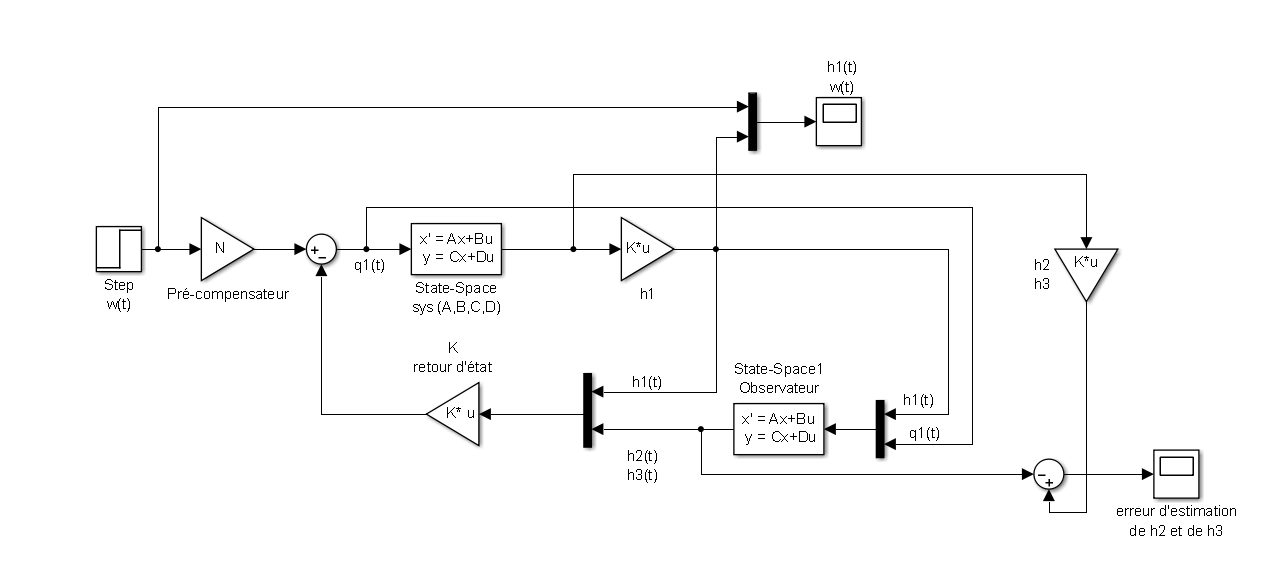
\includegraphics[scale=0.35]{observateurSIMU.PNG} 
		\captionof{figure}{\textit Schéma bloc SIMULINK avec observateur}
		\label{fig4}
		\end{center}
		
		\subsection{\textsc {Convergence des états estimés vers les états réels}}
		
		\begin{center}
		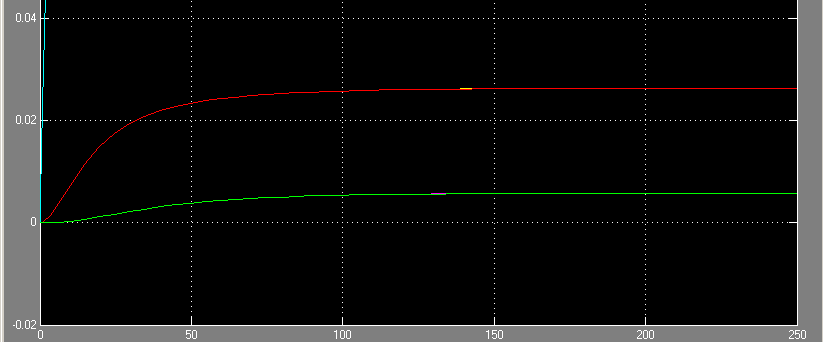
\includegraphics[scale=0.5]{question4.PNG} 
		\captionof{figure}{\textit Courbes d'évolution temporelle des états estimés et les états réels sous SIMULINK}
		\label{fig5}
		\end{center}
		
		\paragraph{} Les courbes $h_2(t)$ et $\widehat{h_2}(t)$ sont identiques, de même pour $h_3(t)$ et $\widehat{h_3}(t)$ donc il n'existe pas d'erreur de convergence en boucle ouverte lorsque les hauteurs initiales sont non nulles. 
		
		\subsection{\textsc {Evaluation de l’influence des conditions initiales de l’état de l’observateur}}

		
		\paragraph{} On prend des conditions initiales de l'observateur de sorte qu'elles soient 50 fois plus grandes que la v	aleur de la consigne.
		
				
		\begin{center}
		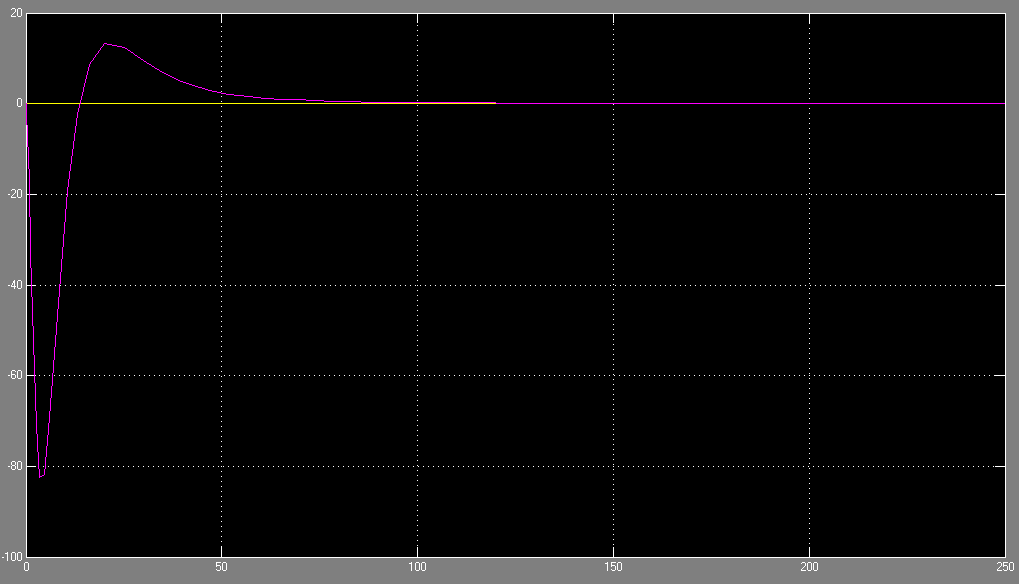
\includegraphics[scale=0.4]{sortiecondi.PNG} 
		\captionof{figure}{\textit Evolution de la sortie après changement des conditions initiales}
		\label{fig6}
		\end{center}
		
		    \textbf{Remarque:} On constate que le dépassement est réduit, il n'y a pas d'érreur de position or le temps de réponse augmente sur la sortie $h_1(t)$.\\ 
		
		\begin{center}
		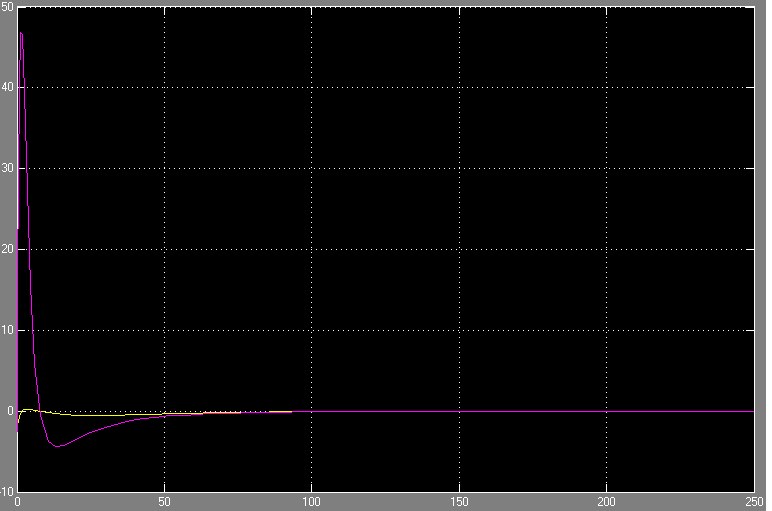
\includegraphics[scale=0.5]{errorcondi.PNG} 
		\captionof{figure}{\textit Evolution de l'erreur d'estimation après changement des conditions initiales}
		\label{fig7}
		\end{center}		
		
		
		\section{\textsc {Bruit sur la sortie mesurée}}
		
			\subsection{\textsc {Courbes de sortie et d'états estimés avec bruit de mesure}}
		
		\begin{center}
		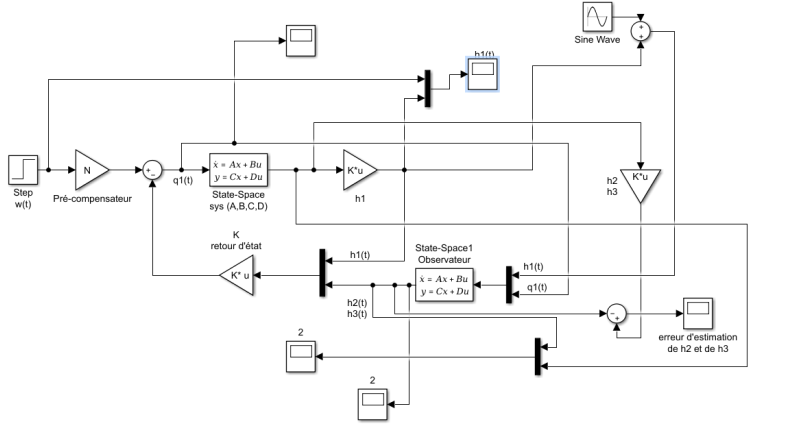
\includegraphics[scale=0.5]{bloc2.png} 
		\captionof{figure}{\textit Schéma bloc SIMULINK avec observateur bruité}
		\label{fig10}
		\end{center}		
		
		\begin{center}
		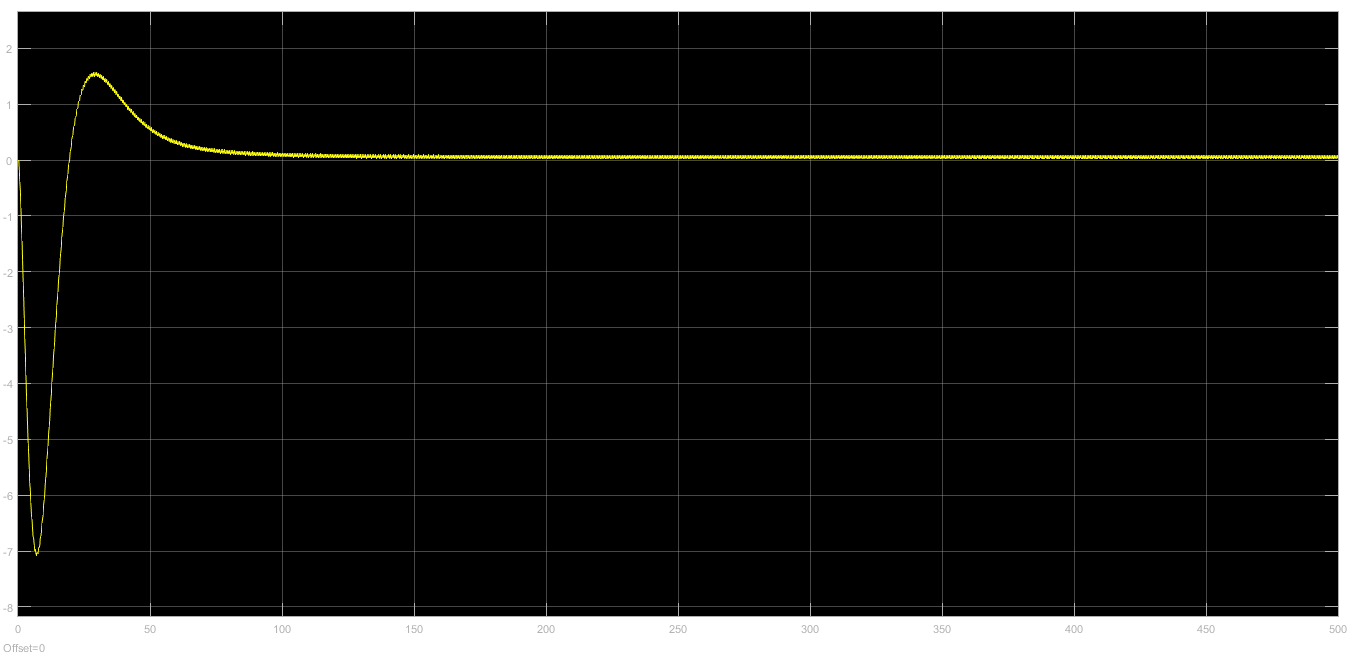
\includegraphics[scale=0.4]{bruit.png} 
		\captionof{figure}{\textit Evolution de la sortie bruitée}
		\label{fig8}
		\end{center}		
	    
		\begin{center}
		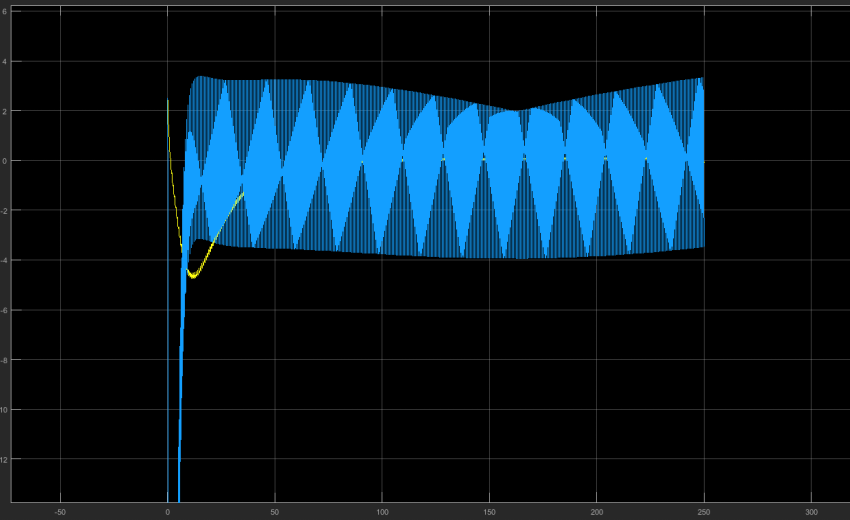
\includegraphics[scale=0.5]{chap5.png} 
		\captionof{figure}{\textit Evolution des états estimés bruités}
		\label{fig9}
		\end{center}		    
	    
	    \paragraph{} Le bruit sinosoïdal $0.001 sin(10t)$ possède un effet direct sur la sortie mais aussi sur les état estimés en ajoutant une composante sinusoïdale qui va les faire diverger. 
	    
	    \subsection{\textsc {Calcul du nouvel observateur}}
	    
	    \paragraph{} Pour cette fois $ P{des} = \begin{bmatrix} 2P_2&2P_3 \end{bmatrix}$, on refait la même procédure que celle de la section 2.1.2 \label{calobs2} \hyperref[Annexe F]{Voir Annexe F}, le système devient alors:
	    
	    \begin{center}
	 $\dot s(t)= \begin{bmatrix} -1.301670&0.010629\\-36.379600&-0.048646 \end{bmatrix} s(t) + \begin{bmatrix} -138\\-5223.66 \end{bmatrix} h_1(t)+ \begin{bmatrix} -9.0455 \times 10^{3} \\ -2.5679 \times 10^{5} \end{bmatrix} q_1(t)$\\[0.25cm]
	 $\widehat{h}(t)=s(t)+ \begin{bmatrix} 139.30\\ 3954.60 \end{bmatrix} h_1(t)$\\[0.25cm]
	 \end{center}
	 
	 \begin{center}
		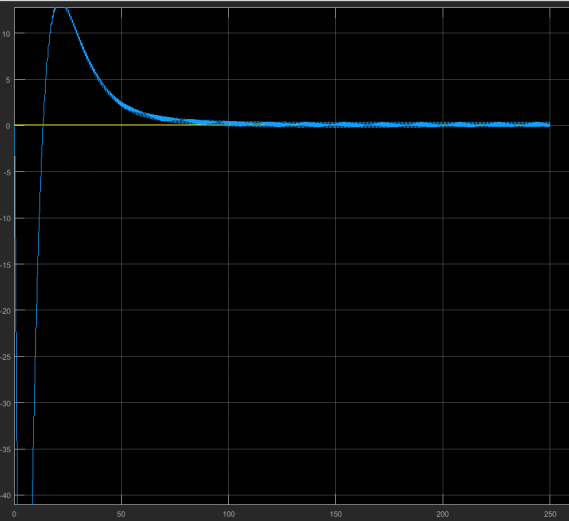
\includegraphics[scale=0.5]{sortie2.png} 
		\captionof{figure}{\textit Evolution de la sortie bruitée du second observateur}
		\label{fig13}
		\end{center}	
		
		
		\begin{center}
		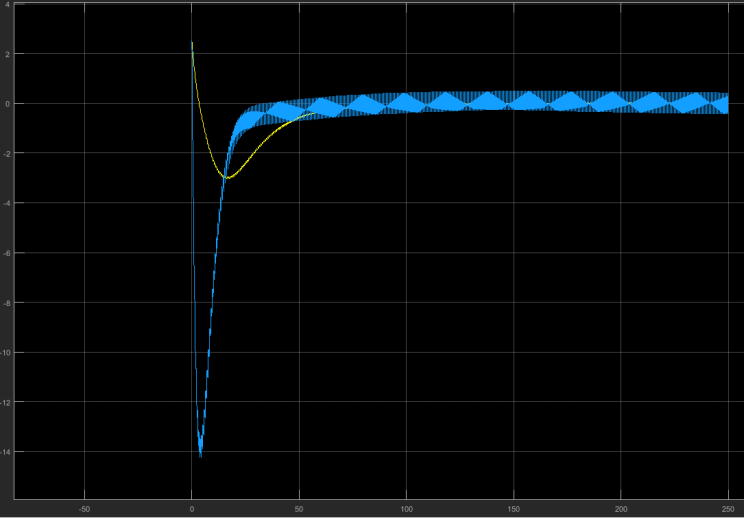
\includegraphics[scale=0.5]{chap2.png} 
		\captionof{figure}{\textit Evolution des états estimés bruités du second observateur}
		\label{fig14}
		\end{center}	
		
		\paragraph{} En effet on constate que l'effet du bruit de mesure diminue en faisant converger le temps de réponse de l'observateur vers celui du système bouclé par retour d'état.